\begin{savequote}
To effectively communicate, we must realize that we are all different in the way we perceive the world and use this understanding as a guide to our communication with others.
\qauthor{Tony Robbins}
\end{savequote}

\chapter[Research Context of This Work]{Research Context of This Work}
\label{ChapterLiteratureReview}


\label{BackgroundFramingClassificationProblem}

%\section{\acf{NVC}}

%\subsection{What is Human Non-verbal Communication?}

\label{BackgroundHowIsNvcExpressed}
\label{BackgroundCompareContrastEmotionWithNvc}

One of the central themes of this thesis is \acf{NVC} and, for clarity, it may be useful to define this term and compare it to the related concept of emotion. \ac{NVC} is the process of communicating by means other than words \cite{Knapp2009}. However, Knapp and Hall \cite{Knapp2009} argued that it is difficult to separate verbal from non-verbal behaviour and to determine if the expression ``by means other than words'' refers to the way \ac{NVC} was expressed, or the interpretation that is assigned by an observer. They did say that the broad but inexact definition will serve, as long as these issues are understood and appreciated. For the purposes of this thesis, communication is considered as an intentional \cite{Jandt2004, Pearce1987} action of exchanging thoughts, opinions or information (which contrasts with the view that communication can be expressed with or without intent). This perspective of \ac{NVC} is similar to Ekman and Friesen's definition of ``communicative non-verbal behaviour'' which they define as ``those acts which are clearly and consciously intended by the sender to transmit a specifiable message to the receiver'' \cite{Ekman1969}. The exact manner in which an \ac{NVC} message is communicated can be carefully planned, or performed without conscious awareness \cite{Knapp2009, Lehtonen1981}. This means that some \ac{NVC} signals are intentionally expressed while the expresser is unconscious of the exact mechanism by which they are expressed. \ac{NVC} can also be defined in terms of behavioural preferences of the communicators themselves, which relates to the use of gestures, posture, touching behaviour (haptically), facial expressions, eye behaviour and vocal behaviour \cite{Knapp2009}.
%Intentionally expressed \cite{Hall2012} \cite{Lehtonen1981}

\ac{NVC} is important for understanding the meaning of communication, because the verbal component is often complemented or augmented by \ac{NVC} \cite{Archer1977, Knapp1978}. Non-verbal signals are often used to regulate a conversation, including turn taking \cite{Kendon1967, Avons1989}. It may be helpful to clarify the terms ``vocal'' and ``verbal''. Verbal means to be or pertain to words, while vocal means to be or to pertain to voice. There can therefore be spoken \ac{NVC} signals, which includes prosody and various non-word utterances such as gasping, groaning, laughing and sighing. The non-verbal component of the voice is also referred to as ``paralanguage''. The audible part of \ac{NVC} is not explored in this thesis, with the focus being on visual, and specifically facial \ac{NVC} signals.

\begin{figure}[tb]
\centering
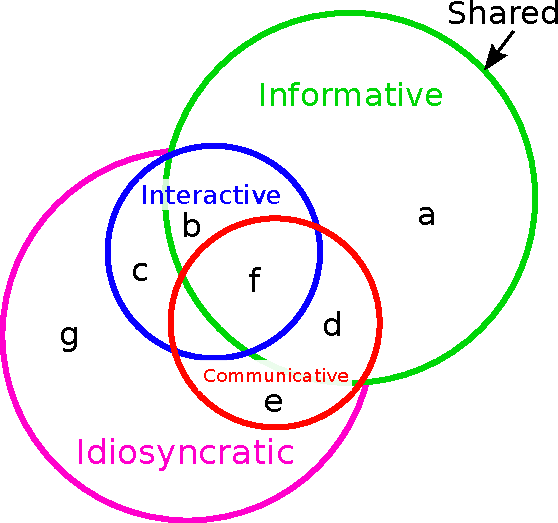
\includegraphics[width = 0.6 \columnwidth]{litreview/EkmanNvb.pdf}
\caption[The relationships between various types of non-verbal behaviours]{A set diagram showing the relationships between various types of non-verbal behaviour, adapted from Ekman and Friesen \cite{Ekman1969}, p. 57. This thesis aims to address communicative non-verbal behaviour, however an annotation's perception of communicative non-verbal behaviour is limited to subsets d and f.}
\label{FigureEkmanNvb}
\end{figure}

This thesis treats non-verbal communication and non-verbal behaviour as distinct concepts (similar to \cite{Krauss1996, Hall2012}), although these terms are sometimes used interchangeably \cite{Negi2009}. Non-verbal behaviours that convey information, called ``informative nonverbal behaviours'' by Ekman and Friesen \cite{Ekman1969}, are defined as acts that ``elicit similar interpretations among some set of observers''. Informative nonverbal behaviour includes both intentional and unintentional transfer of information. A separate issue is if a particular behaviour is communicative, in the sense that the behaviour was intended to be expressed by the sender to convey a particular message. As previously mentioned, Ekman and Friesen defined ``communicative nonverbal behaviour'' as ``those acts which are clearly and consciously intended by the sender to transmit a specifiable message to the receiver'' \cite{Ekman1969}. The terms \ac{NVC} and communicative non-verbal behaviour are treated interchangeably in this thesis and are characterised by their intentional expression \cite{Hall2012, Ekman1969, Lehtonen1981} and the use of a shared decoded meaning \cite{Hall2012, Ekman1969, Lehtonen1981, Wiener1972}. Similarly, Burgoon \etal \cite{Burgoon1996} limited the scope of \ac{NVC} to behaviours that ``are typically sent with intent, are used with regularity among members of a social community, are typically interpreted as intentional, and have consensually recognized interpretations''. An implication of this definition is that some non-verbal behaviours are not communicative \cite{Ekman1969, Engle1998}. Ekman and Friesen define a third type of non-verbal behaviour: interactive non-verbal behaviour which ``clearly modify or influence the interactive behaviour of the other person(s)'' \cite{Ekman1969}. These definitions of non-verbal behaviour are overlapping concepts; the relationship between them is shown in Figure \ref{FigureEkmanNvb}.

In contrast to the definition of \ac{NVC} above, it is popular to define \ac{NVC} in a much broader sense. This view considers communication to encompass all forms of information transfer, including unintentionally expressed behaviour and informative non-verbal behaviour. The broader definition was described by Fiske \cite{Fiske2010} as the ``semiotics school'' and the narrower \ac{NVC} definition (in the previous paragraph) as the ``process school'', with both approaches being necessary for appreciation of the field (see also \cite{Rozelle2006} for a broad literature review). Motley argued that, irrespective of the controversy of definitions, intentional and unintentional behaviour are distinct \cite{Motley1986}. The broad definition excludes the possibility of non-communicative non-verbal behaviour because any behaviour can be potentially interpreted, therefore ``one cannot not communicate'' as claimed by Paul Watzlawick \cite{Andersen1991}. However, this definition was considered to be over-broad by MacKay \cite{MacKay1972}, leading him to joke that by this broader definition, the study of \ac{NVC} would ``cover every interaction in the universe except the use of words!''

%Definition stuff \cite{Thirumalai2003}  \cite{Verderber2007} 
%NVC important \cite{Archer1977} \cite{Knapp1978} \cite{Nakatsu98} \cite{Proyas2004}

Mental state is a broad term for describing temporary mental conditions that have characteristic properties (see \cite{Perner1999} for a review). Mental states include emotion, attitudes, moods and cognitions \cite{Martin1990}. Many mental states manifest themselves as an outward expression and this expression can be intentionally modified to form a partly impulsive and partly controlled expression \cite{Frith2009}. This means mental state displays have both voluntary and involuntary aspects. However, some mental states are not necessarily externally observable, which distinguishes them from \ac{NVC} which is always externally observable. Emotions are a group of mental states that have connections to particular behaviours, have particular physiological manifestations (such as facial expression) and are also subjective experiences \cite{Frijda1986}. They tend to be triggered by stimuli, which are evaluated by a person, and spontaneously results in an emotion. Emotions are often expressed by facial expressions, vocal utterances, behavioural changes, and physical responses. The facial area is particularly important in emotion perception \cite{Ekman2009}. A facial gesture is a motion executed with the facial muscles and may be associated with mental states, emotion or \ac{NVC}. Emotion is an ill defined concept \cite{BeckerAsano2011, Shaver1987, Fehr1984}.
%which lead Fehr and Russell to quip, ``Everyone knows what an emotion is, until asked to give a definition. Then, it seems, no one knows''. 
However, this does not imply that there is no such thing as emotion, nor that it is not a subject worthy of investigation.

\ac{NVC} is a communication act that is only expressed in social situations. While some hold the view that emotions are also limited to social situations, others have observed that some forms of emotion can be expressed in non-social situations such as reading \cite{Mar2008} or dreaming \cite{Nielsen1991}. In a similar way to \ac{NVC} which typically lasting from a few seconds \cite{Lee1998} up to hours or longer, emotions can last from a fraction of a second (e.g. surprise) to hours or even longer (such as with empathy) \cite{Aaron1997, Verduyn2009}. The choice of clothing is an example of \ac{NVC} that has a long duration. A person's internal emotional state is sometimes manifested by facial expression, but the extent to which this is a direct relationship is controversial \cite{Azar2000}. At one stage Ekman claimed that six emotions (Anger, Disgust, Fear, Happiness, Sadness and Surprise) occurred across cultures \cite{Ekman1972} and called them ``basic emotions'', but later appended additional emotions to this list \cite{Ekman99}. He holds the position that different emotions are physiologically discrete and separate. This contrasts with approaches that describe emotions using continuous value labels \cite{Cowie2005}.

A social signal is `a communicative or informative signal which, either directly or indirectly, provides information about ``social facts'', that is, about social interactions, social attitudes, social relations and social emotions' \cite{Poggi2011}. Social signals include `interest, determination, friendliness, boredom, and other ``attitudes'' toward a social situation' \cite{Pentland2007}. The term social signals is used in animal behaviour\cite{Lin2005} and for human non-verbal behaviour \cite{Pentland2007}. The definition does not specify if the signals are necessarily verbal or non-verbal and many authors use the term ``non-verbal social signal'' for clarity \cite{Okwechime2011, Vinciarelli2008}. They are distinct from ``social behaviours'' which ``convey information about feelings, mental state, personality, and other traits of people'' and includes expressions of politeness and empathy \cite{Vinciarelli2008}.
%It is unclear if agreement is a social signal \cite{Poggi2011b} or rather a social behaviour \cite{Vinciarelli2008}.
%Emotion definition \cite{Frijda1991} \cite{Azar2000} \cite{Darwin2002} \cite{Fasel2003} \cite{Frith2009} 
The next section discusses the factors on which \ac{NVC} expression depends.

\section{What Factors Influence \ac{NVC} Expression?}
\label{BackgroundWhatFactorsInfluenceNvc}

There are many factors that influence human expression and perception, and specifically \ac{NVC}. If an automatic system is intended to be trained and deployed in a single environment, this will be of little concern. Although encoding based on motion is not sensitive to context, a system that is to recognise communicative intention for multiple people, or in multiple social and cultural situations, needs to account for contextual factors that can change how \ac{NVC} messages are interpreted\footnote{``From this example, it is obvious that in order to determine the communicative intention conveyed by an observed behavioural cue, one must know the context in which the observed signal has been displayed'' \cite{Pantic2008}}. \ac{NVC} is largely determined by the social situation in which it is used and therefore it is important to study \ac{NVC} in natural social situations \cite{Bavelas97}. Social context is also a factor that is used by human observers to interpret the behaviour of other humans, and humans are not reliable observers when this context is removed \cite{Hoque2009}. Social context, also referred to as social environment, ``encompass[es] the immediate physical surroundings, social relationships, and cultural milieus within which defined groups of people function and interact'' \cite{Barnett2001}. A waving gesture can be a greeting or a sign of distress depending on the context in which it occurs. Although cultural differences in expression exist for many \ac{NVC} signals, some signals have a similar appearance across cultures and social situations. There has been little research of the automatic recognition of \ac{NVC} messages that are specific to contexts, with most existing approaches only considering a single context or seek to generalise \ac{NVC} across different contexts.

%Context important, don't see how this particular paper is relevant \cite{Mower2009}

Factors which influence the expression and interpretation of human behaviour include:

\begin{itemize}
 \item culture (this is discussed in depth in Section \ref{BackgroundCrossCulture}),
 \item gender,
 \item personal style,
 \item personality and
 \item social situation.
\end{itemize}

People naturally vary in expressiveness; some individuals being animated while others being comparatively inexpressive \cite{Afzal2009}. Buck claimed that encoding and perceiving accuracy for \ac{NVC} was dependent on gender, personality and age \cite{Buck1979}. However, these studies assume that there can be ``correct'' and ``incorrect'' interpretations of emotion and \ac{NVC}. This view seems questionable because the use of posed behaviour does not necessarily imply that the samples are directly associated with an objective, exemplar basis of human behaviour. However, the study does highlight the differences in the interpretation. Gender difference in expression style was investigated by Morrison \etal \cite{Morrison2007}, who found there were specific facial movement styles that could be used by humans to identify gender. Some medical conditions, such as schizophrenia spectrum disorder, can change how \ac{NVC} is expressed \cite{Brune2009}. %A study of \ac{NVC} expression in wild chimpanzees also shows individual and age based variations in gesture repertoire \cite{Hobaiter2011}, which is notable because chimpanzee emotional behaviour is comparable to human behaviour except for the lack of verbal communication. 
All these studies provide evidence that there are individual variations in how \ac{NVC} or emotion is expressed.

% 
When humans experience emotion, the emotion often manifests itself in body language and facial expression. Emotion expression is based on many factors. The mapping from emotional state to emotional expression can be thought of as a set of rules, according to Ekman and Friesen \cite{Ekman1975} with each culture having a specific set of encoding rules. Other researchers have extended this idea to specific social situations having distinct display rules \cite{Feldman1991, Brinton2007} that encode the internal state. For this reason, a person expressing an emotion is sometimes referred to as an ``encoder''.
%Matsumoto \etal \cite{Matsumoto08} conducted cross cultural studies and found display rules had commonalities and differences across various cultures. However, cultural differences in gaze aversion was described in terms of cultural rules by McCarthy \etal \cite{McCarthy2006}. 
Research related to the effect of culture is described in more depth in Section \ref{BackgroundCrossCulture}.
Studying the mapping from emotion to expression across cultures can be challenging. To demonstrate that cultural display rule differences or similarities exist, the underlying emotions used must be shown to be equivalent across cultures. \ac{NVC} expression may also have encoding rules which are analogous to encoding and display rules. %However, the terminology of encoding and decoding rules is less commonly applied to \ac{NVC}.
Just as emotions have shared social norms and expectations that are used when managing and modifying emotional displays in different social circumstances, \ac{NVC} expression is also dependent on social circumstances.

%Cross species: \cite{Fridlund94}, \cite{Darwin2002}, \cite{Ekman2009}, \cite{Hobaiter2011} 
%Personality and career choice are associated \cite{Vuust2010}, which leads to personality based perception differences.
%Subjects given shock or no shock, then asked to rate \ac{NVC} of other subjects \cite{Lanzetta1970}, 
%Classifying full body motion with emotion labels \cite{Bernhardt07}, 

Social situation is also a factor in \ac{NVC} and emotion expression. The effect of social situation itself shows cultural, gender and personality differences \cite{Argyle1994} making these factors interdependent. Social situation is significant for capturing a corpus of \ac{NVC} behaviours, because the situation in which the recording takes place affects the type and frequency of observed behaviours. It is often convenient to record posed data, because behaviours directly correspond to pre-determined labels and little time is wasted on recording uninteresting behaviour\footnote{Even if acted data is considered as having no social context, the absence of a social context is a factor in \ac{NVC} expression.}. All human behaviour occurs in a situational context, although acted behaviour may be a special case in that it has a context in terms of social interaction with the audience. Unfortunately, human behaviour is significantly different in posed situations when compared to spontaneous behaviour. Cowie \cite{Cowie2005} argues that the use of posed data cannot be completely excluded but posed data should not be used uncritically. There has been a recent shift in the automatic human behaviour recognition community to use natural data, rather than posed. However there is a wide range of approaches to collect so called ``natural data'' to the point that the word can be misleading. The definition of natural language proposed by Stubbs \cite{Stubbs1983} can be adapted to suit \ac{NVC}: that natural \ac{NVC} occurs ``without any intervention from the linguist [or experimenter]'' and ``is spontaneous in the sense of unplanned, and which is composed in real time in response to immediate situational demands''. Applying this to \ac{NVC}, this definition excludes posed examples of \ac{NVC}, as well as \ac{NVC} based on artificial tasks, stages scenarios, role play tasks or experimenter controlled stimuli (such as a ``Wizard of Oz'' apparatus). The issue of social situation is discussed in more depth in Section \ref{BackgroundSocialContextUsedInTwoTalk}. Just as the expression of \ac{NVC} depends on many factors, the perception of \ac{NVC} is also dependent on multiple factors. These will be discussed in the next section.

%Language word order doesn't seem to change \ac{NVC} order \cite{SusanGoldin2008} although the situation in mime is rather different to natural?

\section{Perception of \ac{NVC}}
\label{BackgroundWhatFactorsInfluenceNvcPerception}
\label{BackgroundPeopleVaryInExpression}

The interpretation of emotion is based on various contextual factors, such as culture, social situation, age, etc. Building on the idea of encoding rules, Argyle \cite{Argyle1994} suggested there exists a mapping from observable behaviour to a meaningful interpretation and termed this mapping as ``decoding rules''. Several studies have found context and conditions that affect perception of human behaviour, including \ac{NVC} and emotion. Terracciano \etal \cite{Terracciano2003} found there is a relationship between personality and emotion perception. Matsumoto \etal \cite{Matsumoto2000} claimed that accuracy in emotion recognition was correlated with personality measures such as Openness and Conscientiousness. Personality differences of experimental participants, such as neuroticism, were associated with different subject gaze patterns being observed during an emotion recognition task \cite{Perlman2009}. However, little work has been conducted in the association between personality differences and \ac{NVC} perception. Behaviour mirroring, which is the tendency of people to adopt the behaviour of another person in a conversation, is more pronounced in people who had tested highly on an empathic personality measure \cite{Chartrand1999}. Lanzetta and Kleck \cite{Lanzetta1970} found that a person's \ac{NVC} perception ability was related to personality and that highly able subjects were themselves difficult subjects for others to read. All these findings provide evidence that both personality and individual style have a role in the perception of emotions and \ac{NVC}.

% The role of personality is thought to influence the choice of career, although that role not well understood \cite{Vuust2010}. 

Another factor in behaviour perception is gender. Vassallo \etal \cite{Vassallo2009} found that gaze patterns during evaluation of emotion were different between genders and that females arrived at a judgement faster than males. Gender based differences in annotator judgements have also been observed in several studies \cite{Buck1979, Terracciano2003, Abrilian2006}. Context can be a factor in perception, but this may still be specific to certain cultures and personalities. The way face images are viewed can affect perception. The presence and expression of surrounding faces changes the judgement of a central face in some cultures but not others \cite{Masuda2008}. Goren and Wilson \cite{Goren2006} found that intense, posed emotion is easier to categorise than weak, posed emotion, as well as finding that emotions are harder to rate accurately if viewed by peripheral vision. Perception of emotion was significantly affected by the level of familiarity with the person being observed \cite{Hoque2009}. El Kaliouby \etal \cite{ElKaliouby03} found that while basic emotions (Ekman 6 and contempt) were almost instantaneously recognized by humans, temporal context improved human recognition for complex emotions, such as interest, boredom, confusion, etc. All these factors make annotation a challenging task, because these variables cannot be easily controlled while maintaining the naturalness of the data. Using multiple annotators and finding a consensus is one common approach. However, personality, relationship and familiarity of people in a social situation are important contextual factors in the expression of \ac{NVC} and using a consensus score discards this aspect of context.

%Perception of hearing is coupled with sight \cite{McGurk1976}

%\cite{Fernandez-Dols2003}, \cite{Reidsma2008Thesis}, \cite{Reidsma2008}, \cite{Eckhardt2009}, \cite{Frith2009}, 

%Perception in context \cite{Archer1977}, \cite{Cowie1999}, 

%\subsection{Models of \ac{NVC} and Emotion}

%Why care about this? Is later discussion sufficient?

%Taxonomies: \cite{Ortony1988}, \cite{Bavelas97}, \cite{Cowie1999}, \cite{Scherer1999}, \cite{Darwin2002}, \cite{Hillard03}, \cite{Jandt2004}, \cite{Darn2005}, \cite{Harrigan2005}, \cite{Matsumoto2006}, \cite{Verderber2007}, \cite{Zara2007}, \cite{Vinciarelli2008}, \cite{Cowie2009b}, \cite{Ekman2009}, \cite{GaticaPerez2009}, \cite{Knapp2009}, \cite{Mower2009}, \cite{Truong2009}, \cite{Wollmer2009}, \cite{Griggs2010}, \cite{Hobaiter2011}.

%Labels: Basic emotions \cite{Ekman1972}, \cite{Ekman1975}, \cite{Matsumoto1990}, \cite{Argyle1994}, \cite{Rosenblum1996}, \cite{Ekman99}, \cite{Cohen2000}, \cite{Marsh2003}, \cite{Feng2005}, \cite{He2005}, \cite{Hong2006}, \cite{Kanaujia2006}, \cite{Datcu2007}, \cite{Moore07}, \cite{Jack2009}, \cite{Moore2009}, \cite{Vassallo2009}, \cite{Fanelli2010}, \cite{Griggs2010}, \cite{Jeni2011}, \cite{Pfister2011b}.

%Abstract scales \cite{Ekman99}, \cite{Cowie2000}, \cite{Liscombe2003}, \cite{Fontaine2007}, \cite{Grimm2007}, \cite{McRorie2007}, \cite{Kanluan2008}, \cite{Truong2009}, \cite{Nicolaou2011}

\section{Supervised Learning for \ac{NVC} Recognition in Video Sequences}

One of the aims of this thesis is to create an automatic system to perform facial, intentional \ac{NVC} recognition, based on previously observed examples of behaviour. As well as directly relevant studies in the field of automatic behaviour recognition, this review discusses research from other fields if they are particularly relevant to this thesis. Video recording of \ac{NVC} has been previously been used in the behavioural sciences \cite{Matsumoto1991}, as well as studies into facial biometrics \cite{Goswami2010}, automatic lip reading \cite{Ong2011}, character animation \cite{Bickel2008} and affective computing systems \cite{Pantic2008, Bartlett2010, Zeng2009}.

Based on video of facial behaviour, training data and manually annotated labels are used to create a model; this process is known as supervised learning. Based on the model, labels for unseen samples can be automatically predicted. The input data and labels are digitised to allow computers to process the input data. Supervised learning is often divided into \featureGeneration, which provides a set of higher level features, followed by a classification technique. 
%Feature generation is also called a feature transform methods, feature construction or feature extraction in the literature \cite{Torkkola2003}. 
Given an ideal training set with total coverage of the feature space, the use of \featureGeneration and a sophisticated classifier would not be necessary; nearest neighbour classification \cite{Cover1967} would be sufficient. However, the available data sets contain a limited number of samples and also contain noise. To improve the performance of a classifier on limited training data, visual changes that are not relevant to the task at hand should be separated or removed from the input data. This improves the robustness of an automatic system and is usually achieved by manual design of the system or by feature selection. This is often accomplished by \featureGenerationComma which aims to improve robustness and reduce the quantity of training data required. Almost every application of supervised learning uses \featureGeneration which transforms the data into a ``higher level'' representation; common approaches are described in Section \ref{BackgroundEncodeFacialInfo}. The \featureGeneration technique used in an automatic system is usually selected manually. There are also many supervised classification methods (described in Section \ref{BackgroundSupervisedClassification}). The type of classifier used may dictate which \featureGeneration approach is optimal and visa-versa, so these issues are closely interrelated. %Manually selecting an appropriate \featureGeneration method and classification technique is necessary because prior knowledge of the problem domain must be exploited \cite{Wolpert1996}.

\begin{figure}[tb]
\centering
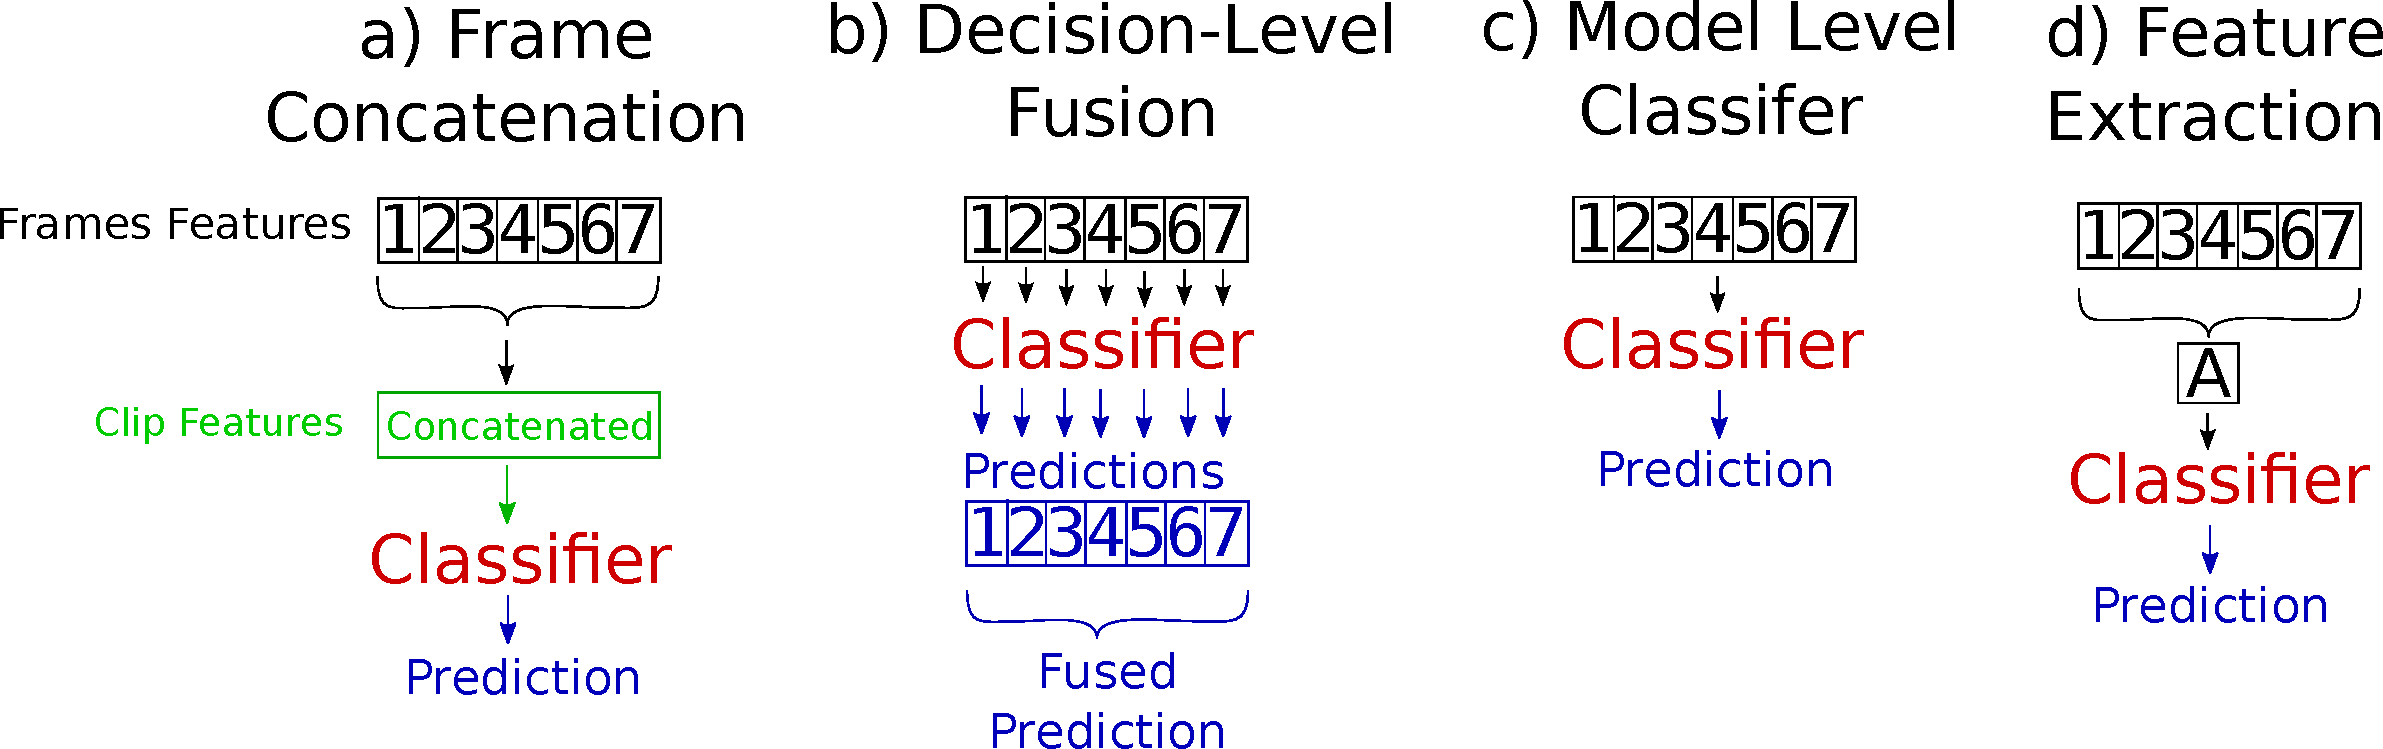
\includegraphics[width = 0.9 \columnwidth]{nvcclass/VideoRecognition.pdf}
\caption[The common approaches to using a classifier with video sequences.]{The common approaches to using a classifier with video sequences. \FeatureGeneration and machine learning have a different role in each case.}
\label{FigureVideoRecognition}
\end{figure}

Once \featureGeneration has been performed on a sequence of video frames, the variable length of examples and temporal nature of a video must be considered to achieve effective automatic recognition performance. This section only considers the processing of visual information and does not consider the issues of fusing audio and video, which is beyond the scope of this thesis. A temporal \ac{NVC} signal can be recognized using data from multiple observations by using \dataFusion which encodes temporal variations early in the recognition process. Alternatively, a model based recognition system may be used, which deals with temporal variation at a higher level.
%Data fusion, or more strictly speaking ``information fusion'', is the exploitation of ``the synergy in the information acquired from multiple sources [...] such that the resulting decision or action is in some sense better [...] than would be possible if any of these sources were used individually [...]'' \cite{Elmenreich2002}. Data fusion is usually used to combine different modalities of data, but may also be used to combine features of a single modality \cite{McKee1993, Zhang2004, Dietrich2001, LakshmiDeepika2009}. 
\DataFusion of multiple observations that were acquired at different times is referred to as ``temporal fusion'' \cite{Varshney1997, Ko2008}. 
%There are different levels of fusion, including: sensor level fusion, feature level fusion and post classification ``expert fusion'' \cite{Poh2010}. Post classification fusion methods include match score level, rank level or decision fusion methods \cite{Poh2010}. Many of these approaches can also be considered as temporal fusion. 
These \dataFusion approaches will now be described in more detail, in the context of temporal, uni-modal video based recognition (see also Figure \ref{FigureVideoRecognition}).

\begin{itemize}
 \item Sensor level feature extraction consolidates raw video image images into a combined raw feature. This is rarely used in the context of human behaviour recognition.
 \item In one form of temporal feature extraction, all frames can be concatenated and directly used by a standard classifier. This can be directly applied to fixed length examples. (Figure \ref{FigureVideoRecognition} a) Frame concatenation is a special case of feature-level encoding. If different modalities are sampled at different frequencies or if samples are of varying length, re-sampling can enable feature concatenation.
 \item Decision level fusion: Each frame can be classified individually using standard machine learning, then the predictions combined and used in a second classifier step to provide an overall overall clip prediction. Decision level fusion may use multiple samples from one or more types of sensor \cite{Vakayallapati2011}. (Figure \ref{FigureVideoRecognition} b). Variants of decision level fusion include rank level fusion and match score fusion. Rank level fusion: multiple recognisers rank possible hypotheses and these rankings are combined to form a final label. Match score fusion: prediction labels are provided by multiple recognizers based on multiple, individual observations and these labels are then combined to generate information for decision making.
 \item Model level recognition: individually encoded frames can be directly used by some types of machine learning methods. The order of the frames in the clip can be used (as typically done with \ac{HMM}, \ac{CRF}) or ignored (e.g. as Nearest Neighbour or \ac{MIL}). (Figure \ref{FigureVideoRecognition} c)
 \item Feature extraction methods 
 %are often used to combine samples of different modalities, but may also be used to fuse features of the same modality \cite{Zhang2004}. They also may 
 encode how low level observations vary over time in a way that can be interpreted by a classifier. Frames can be summarised or combined into a fixed length vector, then classified using a standard supervised learning technique. This approach is used in Sections \ref{SectionTemporalFeatures} and \ref{SectionClipFeatureExtraction}. (Figure \ref{FigureVideoRecognition} d). One simple approach is to concatenate frames into a single vector (Figure \ref{FigureVideoRecognition} a). 
\end{itemize}

Concatenating frame based shape or appearance features before classification is rarely used because videos of varying lengths cannot be directly compared and the approach tends to be sensitive to the speed of activity in the video. For varying length videos, one approach is to re-sample the frame features to produce a fixed length vector, as done by Pfister \etal \cite{Pfister2011}. However, the feature vector can be sensitive to whether an event of interest occurs at the start of a clip, or at the end; this may not be desirable if the occurrence of the event at any time is of significance. This is not an issue for approaches that use unsegmented videos \cite{Oikonomopoulos2011}.

Feature extraction is a popular group of approaches that combine one or more frames into a feature vector, usually of fixed length. Multimodal feature extraction by up-sampling video features and concatenating them with audio features was performed by Petridis and Pantic \cite{Petridis2008, Petridis2009, Petridis2011} and others \cite{Potamianos2001, McCowan2005, Nicolaou2011b}. This can increase the dimensionality of the data, which may reduce the performance of the final system. Other feature-level extraction approaches try to encode temporal variations \cite{Dietrich2001}. Valstar \etal \cite{Valstar2006} calculated the mean and maximum change in the displacement and velocity of feature points during facial deformations, which is a form of temporal feature extraction at the feature level. This reduces the dimensionality of the data while hopefully retaining temporal information about the face. In a similar way, face deformation based on heuristic features was encoded by taking the variance of each feature by Datcu and Rothkrantz \cite{Datcu2007}. As well as using the mean and standard deviation of features in a clip, Petridis and Pantic \cite{Petridis2008} fitted a quadratic curve to each feature component to encode temporal variation. Most of these approaches use geometric deformation based features, however temporal encoding has also been used for texture and audio. Aligned facial textures were compared using the mean shape and appearance features by Fang and Costen \cite{Fang2009}, however, using only the mean does not encode temporal variation information. For audio features, Grimm \etal \cite{Grimm2007} used seven simple statistical measures on the features, as well as the feature's first and second derivatives, which may be useful in encoding the rate of feature variation.

Fusion after matching combines the predictions from multiple classifiers to form a final decision. This is also known as match score fusion and is a form of decision level fusion. This may be used to combine different types of features, different modalities, predictions from independent video frames or the predictions of different classification methods. The most popular decision level fusion methods are the ``sum rule'' and rank based voting \cite{Kittler2003}. The sum rule takes the class dependent average of the predicted probabilities and selects the class label with the highest score. Rank based fusion has each classifier rank each label and these are combined, using one of several approaches, to form a final prediction. One ranking fusion method is majority voting, which takes the highest probability label from the classifiers and the label with the highest proportion is taken as the fused prediction. Audio and visual decision level fusion has been used in many studies \cite{Vakayallapati2011, Poh2010, Petridis2008, Petridis2010, Kanluan2008}. Pfister \etal \cite{Pfister2011b} used majority voting to combine predictions of three types of classifier for visual features. Three different rank based fusion methods were compared by Akak{\i}n and Sankur \cite{Akakin2011} to combine different types of visual features, although there were no appreciable performance differences between the ranking approaches. Audio and video modalities were fused at the decision-level by the sum rule by Petridis and Pantic \cite{Petridis2008}. The sum rule allows the decisions to be weighted to change the emphasis on different modalities, as done manually by Kanluan \etal \cite{Kanluan2008}, or automatically by \ac{LLR} fusion as performed by Lucey \etal \cite{Lucey2009}. Oikonomopoulos \etal \cite{Oikonomopoulos2011} used voting to combine information from different human action models. Ko \etal \cite{Ko2008} showed that dynamic time warping can result in a higher performance than a \ac{HMM} approach for recognizing hand gestures based on multi-sensor fused data. Based on these studies, combining multiple modalities with decision-level fusion often results in a large increase in performance compared to a single modality (although exceptions exist to this pattern \cite{Nicolaou2011b}) and often has recognition performance advantages over feature level fusion (although some studies have shown that the performance using feature fusion is comparable to other approaches in some cases \cite{McCowan2005, Petridis2008}).

Rather than combining features or decisions, feature vectors from multiple frames may be considered directly by a machine learning algorithm. There are two general classes of algorithms: sequential temporal model classifiers (e.g. \ac{HMM}, \ac{CRF}) that consider an ordered group of items, and ``unordered set'' classifiers (e.g. \ac{MIL}) which considers a set of items in which the ordering is not considered. These are among the most popular approaches in the recognition of human behaviour. They are discussed in more depth in Section \ref{BackgroundSupervisedClassification}.

Petridis \etal \cite{Petridis2010} used a different approach to combining multimodal information by using the audio mode to predict the expected visual features and visa-versa. A positive prediction is made if the predicted features match the observed features and this approach exceeded feature level fusion performance for laughter vs. speech discrimination.

\thesiscomment{DISCUSS going via a known intermediary representation e.g. FACS? Emphasis similarity in approach?}

%This section has examined different high level frameworks for human behaviour recognition, and in particular how \featureGeneration and classification are related. The next section will examine the common \featureGeneration techniques.

\section{Encoding Facial Information}
\label{BackgroundEncodeFacialInfo}

\thesiscomment{DISCUSS what part of the body are we trying to encode? ignoring the audio?}

\thesiscomment{DISCUSS features are important \cite{Shan2009} \cite{Yang2009}}

% Almost all automatic approaches use \featureGeneration to encode information about human behaviour. This thesis focuses on facial features, because the facial area is rich in emotion and communication information \cite{Ekman2009}. However, \ac{NVC} signals may be communicated by many other non-facial means, as described in Section \ref{BackgroundHowIsNvcExpressed}. 
Facial features encode shape information by shape or appearance changes, or by combining both types of information. The common approaches will now be described and some of their strengths and weaknesses will be discussed.

\subsection{Encoding Behaviour Using Appearance Based Features}

Changes in facial expression often cause changes in facial appearance due to wrinkles, deformations that change the visibility of the inside of the mouth, etc. However, to make effective use of limited training data, images are typically aligned to a canonical head position or to a canonical head shape. This ensures correspondence between local areas of different face images is maintained and the effect of head pose changes and translation is reduced, making the method much more effective. An alternative is to use changes in an overall image without using alignment which would be effective in encoding head movements, as done by Escalera \etal \cite{Escalera2009}, but this cannot accurately encode subtle facial deformations. Some papers on emotion recognition deliberately ignore the image alignment problem and instead focus on the robustness of later steps in the automatic process \cite{Shan2009}. %Image alignment approaches can be broadly split into part based (or landmark) detection based methods and methods that employ an overall face model \cite{Yang2009b, Boom2010}. 

Some approaches to face alignment begin with interest point detection; the face can be subsequently re-scaled or affine transformed to a canonical alignment \cite{Zhu2009b}. Yang \etal \cite{Yang2009b} used SIFT interest points and a similarity transform. Yang and Bhanu \cite{Yang2011} found point correspondences between images using the SIFT-flow technique and removed shape information in the alignment process. This would help to reduce the effect of identity in emotion recognition. Zhu \etal used Lucas-Kanade based local correspondences to perform a non-rigid transform \cite{Zhu2009b}.

Other approaches for face alignment use whole face detection or a more general model for the overall face shape or colour. The most popular basis for face alignment is the Viola and Jones object detector \cite{Viola2002}, with several studies using this as a basis for image alignment \cite{Kanluan2008, Bartlett2006, Moore07}. Skin colour based detection was used by Feng \etal \cite{Feng2005} to align images; this was robust to illumination changes and, to a limited extent, to pose changes. Some models attempt to fit an expression model (which is often inspired or validated using \ac{FACS} \cite{Cosker2010, Ahlberg2001}) or a shape and appearance model to the observed face, or be limited to variations of shape, head position and pose. Shape based approaches will be discussed below in more depth but there are a few studies that use face models for the purposes of alignment pre-processing before extracting appearance based features. Pfister \etal \cite{Pfister2011} used an active shape model to achieve alignment. \ac{AAM}s may also be used for normalisation \cite{Lan2009} but it common to use the model's parameterisation directly for recognition, rather than to the normalised face as a preprocessing step. Dornaika and Davoine \cite{Dornaika2005} used a 3{D} head model to not only normalise the face translation and pose, but also to remove shape information from the features. Other whole face based approaches avoid shape models and use image information more directly to determine an appropriate alignment transform. Visser \etal \cite{Visser1999} used \ac{PCA} on training images to perform lip localisation, however this was computationally expensive. The alignment transform may be directly found by the affine transformation of an input image on to a canonical image, by maximising pixel intensity correlation \cite{Tzimiropoulos2011}. Rudovic and Pantic \cite{Rudovic2011} used a shape constrained Gaussian process to fit a facial point based model while retaining an anatomically plausible shape. Dhall \cite{Dhall2011} \etal used \ac{CLM} to normalise head positions for emotion recognition, which fits a parameterised model to landmarked positions based on an ensemble of local feature detectors.

Image alignment is intended to remove appearance variations caused by face translation and pose. Often a simple affine or re-scaling transformation is employed. However, natural conversations contain extreme head poses. Until recently, alignment of images based on detection of facial features over a wide range of head poses was an unsolved problem \cite{Zhu2012}. An affine transform from an input image to a canonical face is challenging because of self-occlusions \cite{Yang2011}. For these reasons, using an approach that depends on face alignment to frontal view may fail at extreme poses.

Once the input image has been aligned, appearance features may be extracted that correspond across multiple faces. Two broad approaches are employed: holistically encoding pixel information or part based methods. These types of appearance based features will be discussed.

\begin{itemize}
 \item Holistic approaches use dimensionality reduction techniques to encode changes in overall pixel intensity. Visser \etal \cite{Visser1999} and Seguier \etal \cite{Seguier2002} performed \ac{PCA} on the lip region of interest. Chew \etal \cite{Chew2012} used shape normalised textures to recognise \ac{AU}s and compared this method to local texture approaches under the effect of noise, on four public datasets. Texture descriptors may be applied to every pixel in the image as the basis for classification \cite{Bartlett2006, Moore07}. If a transform is applied on a per pixel basis, the feature vector may become excessively large. Using histograms of texture reduces the representation to a manageable size and also reduces spatial sensitivity, which may be advantageous in improving robustness to insignificant differences in face shape. Kanluan \etal \cite{Kanluan2008} performed \ac{DCT} on lip and eye pixels. He \etal \cite{He2005} used \ac{ICA} on facial images to find independent modes of variation. These methods are useful for finding low frequency spatial information, which is often more relevant than using individual pixels or high frequency components, which correspond to very small areas or very small changes that are unlikely to be significant on their own. However, changes in individual components of these methods typically correspond to a global change in the region of interest and would involve multiple muscle movements. It is likely that features that do not isolate changes based on individual facial muscles would be sub-optimal. %This is due to the inter-person correspondence between muscles for facial expression, as encoded by \ac{FACS}, is closer in similarity than for the face's visual appearance (due to interpersonal differences e.g. face shape, wrinkles, facial hair, etc).

 \item Rather than encode an overall image, a feature can attempt to encode local texture information near points of interest. This makes localised changes in the face affect only some feature components. As mentioned, this decoupling of the different parts of the face may be useful because it is expected that local changes in the face are useful for recognition. Texture descriptors may be applied to limited regions and encoded using histograms, which provides a more compact representation \cite{Feng2005, Shan2009, Pfister2011, Moore2009, Yang2011, Tingfan2012}. There are several popular texture descriptors used in facial recognition, particularly Gabor filters (\cite{Bartlett2006, Wang2006, Rose2006}) and \ac{LBP} features (\cite{Feng2005, Shan2009, Yang2011, Moore2009}). Recent work has considered layers of texture descriptors. Senechal \etal \cite{Senechal2012} used \ac{LGBP} histograms for \ac{AU} recognition, which are \ac{LBP} operators applied to Gabor filtered images. Tingfan \cite{Tingfan2012} compared using a single layer (Gabor energy filters and \ac{LBP}s) with double layer texture filtering, finding that double layer is more effective in multiple data sets.
%These techniques are effective for constrained, basic emotion recognition. 
\ac{LBP}s were extended to encode temporal variation, and named \ac{LBP}-\ac{TOP}, by Pfister \etal \cite{Pfister2011}, however considering changes on a short time scale, such as consecutive frames, may not be optimal for all facial gestures. \ac{LBP} features are also noted for being relatively robust to illumination changes, and in some forms are also robust to rotation. Other approaches include edge based texture descriptors, such as Moore and Bowden \cite{Moore07} using Canny edge detection to form chamfer images as the feature extraction step. Yang and Bhanu \cite{Yang2011} used \ac{LPQ} features that exceeded \ac{LBP}s performance for emotion recognition on acted data. Jiang \cite{Jiang2011} extended the \ac{LPQ} to consider temporal variation (\ac{LPQ}-\ac{TOP}) and found it exceeded performance of \ac{LBP}-\ac{TOP}.
\end{itemize}

Donato \etal \cite{Donato1999} compared many appearance based approaches and found Gabor features with \ac{ICA} dimensionality reduction was the most effective for facial expression recognition.

\thesiscomment{DISCUSS Facial action dynamical models \cite{Dornaika2005}? combines steps into one?}

As previously mentioned, images are usually aligned before appearance features are extracted. While these features have been successfully employed for many constrained datasets, appearance based features are only as good as the face alignment process, which may be problematic for extreme head pose. Appearance based features encode information about the face that can be used as the basis of classification, but also includes information that is not necessarily relevant. Depending on the behaviour under consideration, these irrelevant appearance differences include facial hair, wrinkles, skin colour, glasses, etc. Although some emotions are associated with colour change in the face, colour information is rarely considered because differences in skin colour make interpersonal facial colour comparisons problematic. Various approaches can be employed to remove personal differences in features (Section \ref{SectionPostProcessingFacialFeatures}). Appearance features also may be non-optimal if significant facial movements occur that do not cause a detectable change in local appearance. 
%Wrinkles only form in larger facial movements and small deformations may be ignored by texture descriptors. 
Facial deformations are expected to be important for automatic \ac{NVC} recognition. For this reason, many approaches attempt to encode face shape directly. The next section will consider these types of features.

\subsection{Encoding Behaviour Using Shape Based Features}
\label{BackgroundTemplateTracking}

Shape based features are used to encode information about facial deformation and head pose. Because many human \ac{NVC} signals are based on body and face gestures, encoding the shape captures this type of information. Shape based features usually involve fitting a model to an observation image. The body part selected for feature extraction and sophistication of the model depend on the task that is being attempted. Various approaches have used simple head models that can encode head pose changes, or both the pose and facial expression. Yang \etal \cite{Yang2009} used a simple 2{D} model to encode the face. Chen and Ji \cite{Chen2011} apply \acl{DBN}s to combine facial tracking with expression recognition in a hierarchical framework. Zhu and Ramanan \cite{Zhu2012} used mixtures of trees with a shared pool of parts to localise faces, estimate pose, as well as locate points of interest in unconstrained photographs. Petridis \etal \cite{Petridis2009} used a 3{D} cylindrical model to track the face, with six degrees of freedom corresponding to translation and rotation. This would not encode facial expression but should be sufficient for gestures based on overall head movement. Dornaika and Davoine \cite{Dornaika2005} used a more sophisticated model including deformation to fit facial expression. Zeng \etal \cite{Zeng2006} used a {3D} model based visual tracker for expression recognition. However, complex models are computationally demanding, have higher training requirements and usually require advanced methods to fit the model reliably and robustly. Other approaches use 3{D} shape based on structured light capture systems for emotion recognition \cite{Sandbach2011, Fanelli2010b, Chen2011}. The face is of most interest for \ac{NVC} recognition, but may be complemented by other parts of the body. Occasionally other parts of the body are used for model fitting and recognition, including the shoulders \cite{Petridis2009} or the overall body pose \cite{Bernhardt07}.

Some studies use a hybrid approach to extract a model, such as \ac{AAM}s, and then use only the components corresponding to the shape for recognition \cite{Girard2011}. This has been done by heuristic feature extraction from \ac{AAM} features \cite{Datcu2007}, as well as distance ratios of points of interest \cite{Tang2007}. Other approaches use both shape and appearance, which will be discussed in the next section.

Another approach is to treat the body as independently moving parts, localise the position of each part in the frames of the video sequence and use this information directly, or fit a model based on the independent parts. This is conceptually simpler than fitting a complex model with inter-dependent parts. However, position and motion of areas of the body can provide information for the movement of nearby body areas and this is not used by tracking independent points of interest. Tracking attempts to localise a feature of interest in a series of video frames. Tracking uses the assumption that a point of interest has a locally constant appearance. This separates motion from other non-shape changes in the video. However, large changes in appearance caused by pose changes or occlusions make tracking spontaneous videos difficult. Lucas and Kanade  \cite{Lucas1981} proposed a method based on minimising the least squares difference of a training patch to a test image by gradient descent. However, it can suffer from local minima, noise and occlusions which can lead to tracker drift. An alternative is to use a particle filter based approach, which is robust to noise by using multiple hypotheses of tracker position \cite{Isard1998}. However, this approach does not scale well to high dimensionality. This was addressed by partitioning the model space components into groups by Patras and Pantic \cite{Patras2004}. This tracking method is limited to small head pose changes of approximately 20 degrees \cite{Valstar2012}. This is because of the change of appearance caused by head rotation breaks the assumption of an unchanging local appearance near to a tracked point of interest. Chew \etal \cite{Chew2012} used a \ac{CLM} to detect \ac{AU}s, which uses detections of facial points of interest as the basis to fit a shape model. \ac{CLM}s \cite{Cristinacce2008} are similar to \ac{AAM}s but generate likely feature templates that correlate with the target image, rather than trying directly fitting a model to pixel intensities. Baltrusaitis \etal \cite{Baltrusaitis2012} extended \ac{CLM}s to {3D} and applied it to head pose tracking. Liwicki \etal \cite{Liwicki2012, Liwicki2012b} proposed a kernel \ac{PCA} method, which retains desirable properties of \ac{PCA} while being robust to outliers; this encodes behaviour as shape information. They applied the method to different computer vision problems, including visual tracking and found it was better than 4 other state-of-the-art tracking methods in most video sequences.

The approach used in this thesis is the pre-existing tracking technique proposed by Ong \etal \cite{Ong2009} called \acf{LP} tracking; this method encodes behaviour as face shape changes. This method learns a linear mapping from intensity changes in a sparse template to a tracker positional offset. The tracker is trained on multiple training frames which improves its robustness to appearance change, including an amount of head rotation. The maximum tolerated head rotation is not known, but it is suitable for tracking spontaneous human behaviour. The tracker does not automatically recover from occlusions, so the tracker must be manually re-initialised when a feature becomes visible. This could be addressed by incorporating an automatic feature detector to re-initialise tracking positions. This tracking process results in the facial behaviour being encoded as a series of shape deformation frames. The technical details of \ac{LP} tracking are discussed in Appendix \ref{BackgroundLpTracking}.

Tracking data encodes facial deformation changes and can be used directly for behaviour recognition. Tracking is not effective in areas which contain relatively little local texture, such as can be seen in puffed cheeks. Tracking has often been applied to estimate optical flow and this approach encodes the overall face deformation. This method was used to recognise emotions by Rosenblum \etal \cite{Rosenblum1996}. Overall head translation information is usually unrelated to facial expression and is often separated from facial deformation information. However, differences in face shape can prevent direct comparison of optical flow features generated on two different people. Also, optical flow based approaches tend to be sensitive to head rotations and require a constant frontal view of the face. Other approaches use tracking of points that corresponds to known positions on the face. This correspondence makes inter-person comparison of deformations easier. Tracker movements are caused by both head movement and expression changes, but this is not ideal for existing machine learning techniques. Head motion was separated from deformation changes using \ac{PCA} by Petridis and Pantic \cite{Petridis2008}. Another way to improve person independent recognition is to remove the effect of face shape by mean shape subtraction \cite{Tax2011}.

%Direct use of tracking features? \cite{Nicolaou2011}

\subsection{Encoding Behaviour Using Both Shape and Appearance}

The previous sections have discussed features that encode either the shape or the appearance of human \ac{NVC} and emotion. To guide future work, it may be useful to know which approach is most effective, or if these approaches can be combined effectively. Some papers compare shape features to appearance feature approaches and this provides insight into the best approach for encoding behaviour. However, comparisons of specific techniques do not rule out the creation of superior \featureGeneration techniques. Lien \cite{Lien1998a} compared three methods (feature point tracking, dense flow and texture descriptors) for emotion recognition of posed examples and found dense optical flow is most effective. Both Fanelli \etal \cite{Fanelli2010} and Akak{\i}n and Sankur \cite{Akakin2011} had similar findings, with optical flow or tracking being effective but optical flow or tracking combined with appearance and shape demonstrating a higher performance. However, optical flow techniques are susceptible to head rotation, which commonly occurs in spontaneous behaviour. Some model based methods extract both shape and appearance information which can be used for recognition. A popular approach for facial analysis is an \acf{AAM} \cite{Cootes1998}. This has been used for emotion recognition and studies have found that while shape is more important than appearance, use of combined shape and appearance has a higher performance \cite{Ashraf2007, Lucey2009}. However, \ac{AAM}s have difficulty fitting to faces under a wide range of poses and expressions, and require additional specialised models to account for this variability \cite{Peyras2008, Lee2009}. This increases the training requirements of \ac{AAM}s, making their application to new subjects very time consuming. Koelstra \etal \cite{Koelstra2010} used motion both history images (which encodes appearance information) and a motion field (which encodes face shape changes) to form local histograms, as the basis for classification of facial actions with motion deformation features being the more effective approach.

%An early work on lip reading by Luettin \etal \cite{Luettin1996} found that lip shape and intensity information provided the same performance, but combining the approaches improves performance. Lip shapes, low pass filtering of mouth pixels better than optical flow \cite{Gray1997}
%Uses ASMs and AAMs on lips, some performance as \ac{MSA} texture descriptor on lip region, \cite{Matthews1998}
%Heuristic \cite{Smith2005}

The FERA2011 Challenge on emotion and \ac{AU}s attempted to benchmark different approaches to provide a clear ranking for current approaches \cite{Valstar2011}. Despite the apparent dominance of shape based features in other comparisons, the best performing approach in this challenge used appearance features on aligned faces \cite{Yang2011}. Several other approaches used fusion of both appearance and shape \cite{Valstar2011slides, Valstar2012b}. Senechal \etal \cite{Senechal2012} used an \ac{AAM} to recognise \ac{AU}s but this was found to be less effective than \ac{LGBP} histograms. Tariq \etal \cite{Tariq2011} fused local optical flow, \ac{SIFT} histograms and Hierarchical Gaussianization achieved the best person-specific emotion recognition performance.

Only a single paper used shape \featureGeneration exclusively but did not have a competitive performance. All the published comparisons of different classes of features have used posed data. The relative importance of shape and appearance is still under debate for this problem, but combining both types of features usually results in improved performance.

\subsection{Encoding Behaviour Using Audio Features}

Paralangauage, which is a form of non-verbal audible communication, provides information that is not necessarily available if only visual facial behaviour is considered. Many studies have employed audible signals exclusively or combined both audio and visual signals (see \cite{Schuller2011} for a review). Audio feature extraction methods include fundamental frequency (F0) \cite{Liscombe2003, Grimm2007}, intensity, Mel Frequency Cepstral Coefficients \cite{Grimm2007}, distribution energy in spectrum \cite{Truong2009}, speech rate \cite{Truong2009} and manually extracted features e.g. spectral tilt \cite{Liscombe2003}. Automatic systems have been created that recognise arousal and valence labelled data \cite{Truong2009}, categorical emotional labels \cite{Liscombe2003, Hassan2009} and affective states \cite{SobolShikler2010}. Hassan and Damper \cite{Hassan2009} showed that finding an appropriate subset of features, using \ac{SFS}, can enable a simple classifier (k-nearest neighbour) can provide a better performance than \ac{SVM} classification without feature selection. Speaker normalisation is sometimes used to improve generalisation to new subjects \cite{SobolShikler2010} or languages not contained in the training data \cite{SobolShikler2010, Hassan2012}.

Many studies use both visual and audio features to recognise behaviour and emotion \cite{Petridis2011, Kanluan2008, Haq2009}. There is a close association between facial behaviour and the non-verbal channel of communication \cite{Busso2007}. The next section describes further processing that can be applied to features, in an attempt to improve robustness.

\subsection{Post-processing of Facial Features}
\label{SectionPostProcessingFacialFeatures}

As discussed in the previous section, \featureGeneration attempts to extract relevant information from raw observations while ignoring variations that are irrelevant for the intended task. Many \featureGeneration approaches consider individual frames and do not consider the overall video sequence. However, facial expressions can evolve over many frames, rather than being restricted to one or two frames. Using the information for multiple frames can be useful to generate better features and to make the final system more robust. Face shape is associated with a person's identity but this is not of interest for automatic \ac{NVC} recognition. Also, individual feature components can be processed by dimensionality reduction algorithms to attempt to isolate the information of interest. This makes the features more suitable for machine learning, particularly when combined with feature selection.

Using the set of feature values over a long time period, various normalisations may be applied. Face shape for neutral expression cannot easily be inferred from a single frame of video because of the possible presence of expression, but over many frames the neutral face shape is relatively easy to determine, particularly in naturalistic behaviour which often contains long periods of neutral face expressions. The effect of face shape can then be subtracted from the features which improves a system's robustness to identity. Other inter-personal differences, such as facial hair, skin colour and glasses can affect appearance based features but can be managed in a similar way to face shape. There have been several different feature normalisation methods proposed including mean feature subtraction \cite{Jeni2011, Tax2011} and scaling features to a standard variance \cite{Yang2009} (also referred to as ``whitening''). Six audio feature normalisation methods were compared by W\"{o}llmer \etal \cite{Wollmer2008} who found that normalising features to a range of -1 to +1 was advantageous in some cases and was thought to remove identity based differences. Such normalisations are suitable for recorded data but cannot be immediately used for prediction based on a previously unseen face. 

\thesiscomment{DISCUSS invariance \cite{Taheri2011}}

Features often encode both information of interest as well as irrelevant information. It can be beneficial to use dimensionality reduction in an attempt to separate relevant information into specific feature components in an unsupervised way. Lien \etal \cite{Lien1998a} used \ac{PCA} on dense optical flow features of the face from multiple frames to produce ``eigenflows''. Fang and Costen \cite{Fang2009} used \ac{PCA} to encode facial feature position motions and Akak{\i}n and Sankur \cite{Akakin2011} applied \ac{ICA}, \ac{NMF} and \ac{DCT} on sequences of facial feature positions. Individual components of features in the eigenvector based methods correspond to deformations of part or all of the face. These deformations are found in an unsupervised fashion and are not necessarily optimal for recognition. Also, the order of events that are encoded in the sequences are either not encoded at all, or encoded in a way that is not appropriate for machine learning. 

\thesiscomment{DISCUSS feature selection, \cite{Bartlett2006}, reference later chapter}

Another important feature processing stage is feature selection, which is discussed in Chapter \ref{ChapterFeatureSelection}. The next section describes techniques for supervised classification based on features.

\section{Classification}

\label{BackgroundSupervisedClassification}

\begin{figure}[tb]
\centering
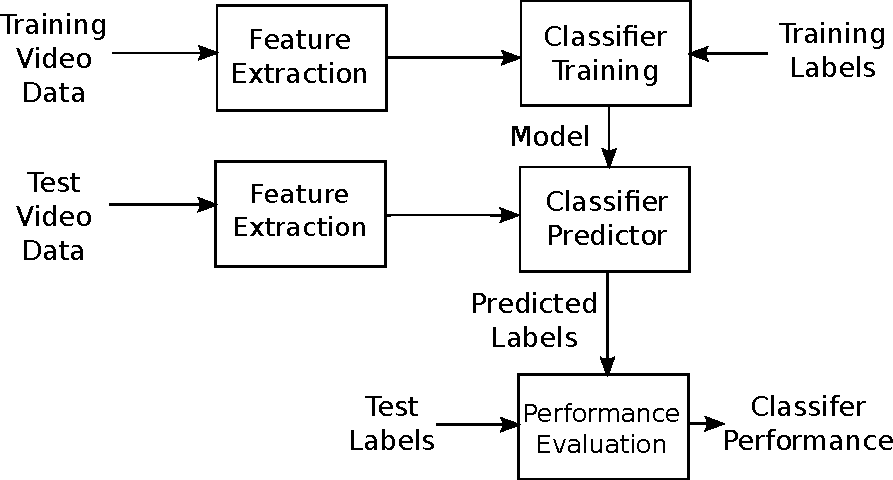
\includegraphics[width = 0.6 \columnwidth]{nvcclass/supervisedSystem.pdf}
\caption{Supervised learning uses labelled training data to create a model that can make label predictions for unseen data.}
\label{FigureSupervisedClassification}
\end{figure}

One of the aims of this thesis is to create an effective automatic system for \ac{NVC} recognition. After feature extraction and processing, the final step in an automatic system is often classification, which is the process of automatic prediction of a label based on a test sample observation. Many different classifiers have been applied to emotion, speech reading and gesture problems. This section provides an overview of the significant existing approaches to classification.

A supervised classifier is used to create a model based on labelled training data. This model can be used to predict labels for unseen test samples. The samples' features are usually the result of a \featureGeneration process from raw observations such as video frames. In this case, a test or training sample is a video clip of one or more frames. Given a set of training and test data, the performance of a classifier can be evaluated by comparing its predictions for unseen samples to the test data labels, also known as ``ground truth''. An illustration of this process is shown in Figure \ref{FigureSupervisedClassification}. There is a vast number of classification techniques in the published literature. Specific disciplines often have a set of preferred techniques that have been found to be effective. This is because each classifier has different requirements and makes different assumptions about the problem's characteristics. Also, each \featureGeneration technique has different properties, so features vary in suitability based on the problem and the specific classifier used. Rosenblum suggested that expressions with greater motion are easier to classify \cite{Rosenblum1996}. This section will focus on the use of classifiers in various facial classification applications and will discuss some of the classifier's properties in each context.

There are a few major families of classifiers, each requiring different formats for the input features and input labels. 
%The most common type of classifier have a single vector as an input feature, and a single discrete value as a label (and this is often restricted to a two class problem). Sequence classifiers, in contrast, have an ordered set of vectors to encode a sample's features. Multiple instance classifiers are similar to sequence classifiers but relax the ordering requirement for the sample's features. Classifiers also vary in that some require the feature vectors to use discrete values and others do not. 
For this reason, it is not possible to apply every classification technique to every problem. 
%Regression techniques are similar to classification techniques but use real values for their data labels. Regression is discussed further in Chapter \ref{ChapterNvcRegression}. 
The main families of classification techniques will now be discussed, along with the problems to which they have been applied.

\subsection{Single Instance Classifiers}

Single instance classifiers operate on samples that are represented by a single feature vector and a label value. This reliance on a fixed length feature vector makes classification of variable length clips problematic, but this can be overcome by \featureGeneration or decision level fusion. An early classifier was based on finding the $k$ nearest neighbours for a test sample \cite{Cover1967}. This approach is conceptually simple but it has high computer memory requirements. It also considers all feature components as equally significant, which can be problematic if some of the components of the feature vector are irrelevant. This may be the case for \ac{NVC} and emotion recognition, because typically only part of the face is relevant in determining the label. Donato \etal \cite{Donato1999} applied the nearest neighbour technique to facial expression classification. Nearest neighbour is appropriate for problems that have a large quantity of training data. Most classification techniques use a statistical model to approximate the decision boundary between different classes in feature space. One of the earliest classification techniques is \ac{FLD}, which attempts to use a linear manifold to separate two classes. Linear discrimination was applied to facial expression by Rose \cite{Rose2006}. 
%The boundary hyperplane can be specified by two points in feature space that are on opposite sides of the manifold and are equidistant from each point on the manifold. For facial features, these feature points corresponds to two exemplar face configurations; one exemplar corresponds to the positive class and one for the negative class. Hong \etal \cite{Hong2006} applied the enhanced Fisher linear discriminant model, which combines \ac{PCA} dimensionality reduction with \ac{FLD} to emotion classification. \ac{LDA} assigns class labels based on a test sample based on their proximity to each of the two samples. Based on this concept, we can see \ac{LDA} simplifies a complex nearest neighbour partitioning of feature space to a very simple partitioning. 
Unfortunately many problems in facial analysis require the use of non-linear decision boundaries to achieve acceptable performance.

\thesiscomment{DISCUSS \cite{Wang2006} using LDA for emotion?}
\thesiscomment{DISCUSS which methods are robust to outliers?}

A neural network is a machine learning technique based on an interconnected group of artificial neurons. Neural networks have high training requirements, and high computational and memory requirements. They also generate an internal model that is hard for humans to interpret and therefore only provide limited scientific insight. Their partitioning of feature space is also hard to grasp intuitively. However, neural networks have been used in a wide range of applications including speech reading \cite{Visser1999, Seguier2002}, emotion recognition \cite{Rosenblum1996, Petridis2009, Wollmer2009}, classifying laughter or no laughter \cite{Petridis2010} and many other non-facial analysis applications.

Boosting classifiers are a family of machine learning techniques that combine a set of weak learners into a single strong classifier. This is usually done iteratively and greedily, with weak learners being weighted and added to a bank of weighted weak learners. Many boosting approaches limited the weak learners to produce Boolean feature vectors and also require Boolean class labels. This makes some boosting methods less attractive if facial deformation features and \ac{NVC} labels can be considered as continuous values. One popular boosting method is Adaboost \cite{Freund1996}, which is a binary classifier known to be sensitive to outliers \cite{Natsuki2008}. Adaboost was applied to emotion classification by Moore and Bowden \cite{Moore07} and He \etal \cite{He2005}. Adaboost has been extended to temporal sequences and this is discussed in the later section on temporal model classifiers. The technical details of Adaboost are discussed in more depth in Section \ref{SectionAdaboost}. Boosting methods often explicitly select a subset of features which is easy to interpret and this can be useful in finding the types of face deformations that are responsible for determining the label of a test sample.

%Omitting Probabilistic Boosting-Tree? \cite{Tu2005} did someone use it? Adaboost was extended to multiclass \cite{Zhu2006}

A \acf{SVM} is a kernel based learning technique that attempts to learn a decision boundary that provides the maximal separation between positive and negative samples (Vapnick \cite{Vapnik1998}). In the input feature space, the boundary is non-linear and allows many complex problems to be addressed but at the risk of over-fitting, resulting in lower performance. The boundary model is based on adding weighted kernels centred at particular training samples. A test sample's distance from the boundary provides a mapping to a SVM space in which the problem is linearly separable. \ac{SVM} was originally formulated for binary classification and have since been extended in various ways, including for regression, which is used later in Chapter \ref{ChapterNvcRegression}.
%The original formulation was based on the two class problem, but various extensions for multi-class \ac{SVM} have been proposed and a compared between them was conducted by Duan and Sathiya Keerthi \cite{Duan2005}.
The \ac{SVM} method is popular and has been applied to facial analysis many times. It has been shown to be effective in emotion classification \cite{Goecke2006, Datcu2007, Seppi2008, Moore2009, Truong2009, Tariq2011, Jeni2011, Yang2011}, classifying pain or no pain \cite{Ashraf2007} and on \ac{AU} based expression recognition \cite{Taheri2011, Girard2011}. However, \ac{SVM}s do not provide an intuitive way to interpret their internal model, or to easily determine which features are most relevant. The technical details of the \ac{SVM} is discussed in more depth in Section \ref{SectionSupportVectorMachines}. A \acf{RVM} is a kernel technique that is closely related to \ac{SVM} but uses \ac{EM} to find a model to provide probabilistic label prediction. However \ac{EM} does not necessarily find a globally optimal model but still is an effective classifier that results in a sparser model and is often seen to result in a higher performance when compared to \ac{SVM} \cite{Nicolaou2011b, Xiangmin2007}. \ac{RVM} was applied to classifying brow action samples as posed or spontaneous by Valstar \etal \cite{Valstar2006}. \acf{SVDD} is another kernel method but in this case addresses the problem of modelling a single class's distribution. This was used by Zeng \etal \cite{Zeng2006} to model samples in one class labelled as ``emotional'' and this was used to classify test samples as either emotional or unemotional. This one class approach is useful if it avoids the problem of attempting to model a class which has a  complex feature space occupancy.

\thesiscomment{CHECK what does it mean when RVM is probabilistic?}

A decision tree classifier learns a graph of simple rules that recursively divide the feature space along axis parallel planes \cite{Breiman1984}. Decision trees are fast to train and apply, they provide a simple way for human inspection of the internal model and allow feature relevance to be determined. Decision trees were applied by Hillard and Ostendorf \cite{Hillard03} to agreement and disagreement classification in audio. Decision trees have been extended to random forests \cite{Breiman2001} in an attempt to improve performance. Random forests use an ensemble of decision trees with each tree trained on a different subset of features, using the concept of bagging. Random forests produce a verbose model that is difficult to interpret, in comparison to decision trees, but relevant features can still be evaluated. Random forests have been applied to emotion classification on posed data \cite{Fanelli2010}.

\thesiscomment{DISCUSS? Linear programming on emotion recognition \cite{Feng2005}, Dynamic Cascades with Bidirectional Bootstrapping on FACS \cite{Zhu2009}, Pair-wise machines on emotion \cite{SobolShikler2010}}

While some approaches to facial analysis have used human designed \featureGeneration, it is uncommon to attempt to manually create a classification model. However manual classification rules were created by Pantic and Patras \cite{Pantic2006} to classify \ac{AU} based facial expression. This allows human technical and intuitive abilities to be applied to the task to produce a tailored model, but this might not be appropriate for complex feature space distributions or in cases where the relevant features are unknown.

The classifier methods in this section have been concerned with samples having a single feature vector. The following section considers classifiers that specialise in modelling temporal and sequential problems.

\subsection{Temporal, Model Level Classifiers}

Temporal model classifiers are trained on samples that have been encoded as features that are an set of vectors. An ordered sequence of vectors is often based on sequential audio features, video frames or gestures in a clip of limited duration. This discussion will focus primarily on video classification, which is the topic of this thesis. Sequential temporal model classifiers attempt to model the temporal variation of features for each class. This model can then be used to predict a label for test samples. The most popular sequential classifier is the \acf{HMM}, which assumes a process can be characterised by transitions in a hidden state model. The transitions between hidden states are assumed to have a Markov property, which means the transition to the next state depends on the current hidden state but does not depend on previous hidden states. Each hidden state is associated with an emission model, which maps a hidden state onto a distribution of observable states. A separate \ac{HMM} is trained for each class, including a class specific hidden state transition model and an emission model. For gesture recognition, the hidden states are usually discrete labels, and the emission model is typically a Gaussian distribution. If features that encode facial expressions are used, each hidden state corresponds with a distribution of facial expressions. A particular class would be characterised by the transitions from one distribution of facial expressions to the next. 

\ac{HMM} is an elegant theory which has been successfully used in many applications. However, there are a number of disadvantages arising from model used and assumptions that are made. The hidden state model usually allows for self transitions to remain in a state. Because of the Markov property, the probability of remaining in one state reduces exponentially in time, and it is difficult to say if this would be appropriate for \ac{NVC}, or not. The emission model is assumed to be a Gaussian distribution which, for facial features, makes certain assumptions as to the properties of facial expression. Many of these issues can be addressed by increasing the number of hidden states in the model, but this quickly increases the number of unknown parameters in the transition model and the emission model. \ac{HMM}s typically operate best when there is a large quantity of training data available. The number of hidden states and the topology of the transitions are difficult to determine without manual adjustment, which makes the application of \ac{HMM}s rather time consuming and heuristic. Also, \ac{HMM}s use discrete class specific models and these cannot directly be used to predict continuous value labels.

\ac{HMM}s have been successful in the other form of human communication: verbal language recognition. Speech recognition often considers only the audible component but some studies have combined audio and visual facial analysis with \ac{HMM}s to improve recognition \cite{Potamianos2001, Nefian2002}. Language recognition can even be attempted with visual only features, although previous studies have been restricted to a limited grammar \cite{Luettin1996, Gray1997, Matthews1998, Saitoh2005}. Another quasi-verbal mode of human communication is sign language, to which a \ac{HMM} classifier has also been applied \cite{Starner1995}. Although almost entirely visual, sign language is generally not regarded as \ac{NVC} because multiple gestures are combined to form complex meanings. The difference between sign language and \ac{NVC} is that sign language has a grammar while \ac{NVC} does not. Emotion is also thought not to have a grammatical structure \cite{Cohen2000}. This lack of grammar makes it unlikely that \ac{HMM}s will be particularly effective for \ac{NVC} recognition. On more constrained problems, such as posed emotion or posed facial expression that begins and ends on neutral expression, a clear pattern of expression onset (appearance), peak and offset (disappearance) \cite{Ekman1984} can be seen. This may serve as a grammar of sorts, which can be used by a \ac{HMM} in facial expression classification \cite{Lien1998a} or emotion classification \cite{Cohen2000, Mower2009}. However, naturalistic emotion and \ac{NVC} does not necessarily begin and end with neutral expression and this reduces the consistency on which sequential temporal model classifiers depend. el Kaliouby and Robinson \cite{Kaliouby2005} use \ac{DBN}s, which are a generalisation of \ac{HMM}s to classifying mental states. Their approach integrates modelling of different temporal and spatial scales into a single classifier.

\thesiscomment{HMM on identity from lip shapes \cite{Mok2004}}

Adaboost was extended to consider temporal sequences as the TemporalBoost classifier and was tested on facial gestures by Smith \etal \cite{Smith2005}. This technique considers frames in a window of variable length, ending with the last frame of the sample. For each boosting iteration, the binary input features in the variable window have a logical ``AND'' and ``OR'' operator calculated, which are the values used for boosting. The variable window size is optimised to minimise the prediction error by gradient descent. As with most boosting methods, the trained model provides informative feature relevance information. Although this classifier considers multiple frames, it does not model how features vary in time in any direct sense. In testing, the order of frames in the window is not considered. Also the classifier is limited in that consecutive frames in a window must be considered, and the window end must correspond to the end of the clip, which makes it inappropriate if significant events occur at the start of a clip. As with Adaboost, TemporalBoost is limited to binary inputs and binary labels which makes it less relevant to continuous value problems.

A \acf{CRF} is a class of machine learning tools that, unlike conventional classification, which considers test samples independently, the label assignment of each sample considers the labels of ``nearby'' samples, which when applied to temporal data corresponds to nearby in time. In classification of video, this can enable a video frame to be classified based on adjacent frame labels. Hidden \ac{CRF} extends this with the addition of a latent, unobserved state. This method, like a \ac{HMM}, has discrete state transitions that are usually considered over short time periods. This may not be suitable for gradually varying human emotion and \ac{NVC} signals. Morency used \ac{CRF} to predict and recognise the behaviour of a human listener \cite{Morency2011}. Bousmalis \etal \cite{Bousmalis2011} used \ac{HCRF} to classify agreement and disagreement in political debates. This was later extended to \ac{iHCRF} \cite{Bousmalis2012}, which is capable of automatically finding the optimal number of hidden states. Rudovic \etal \cite{Rudovic2012} extended the \ac{CRF}-like \ac{CORF} method \cite{Kim2010} to take account of the ordinal relations between onset, apex and offset for \ac{AU} recognition. 

\thesiscomment{DISCUSS that we are classifying clips with a single label, rather than continuously varying sequences?}

Sequential classifiers consider samples that contain a set of ordered video frames. However, the following section will consider classifiers that specialise in classification of unordered sets, which may be appropriate for ``grammar free'' \ac{NVC}.

\subsection{Multiple Instance and Trajectory Classifiers}

\acf{MIL} considers classification of a set or ``bag'' containing one or more vectors or ``instances'' \cite{Maron1998}. This may be applicable to \ac{NVC} recognition, because it is possible that the presence of a single face configuration to be important in determination of the predicted label. If a particular area of feature space is critical to determine the label, it is known as a ``concept'', which corresponds to a specific face configuration. However, \ac{MIL} places minimal constraints or assumptions on the nature of the data, so there is no common \ac{MIL} approach. There are rather many different \ac{MIL} algorithms that have been proposed for domain specific problems. Also, it is unclear whether a single exemplar or concept is sufficient to encompass a range of naturally occurring \ac{NVC} signals. Tax \etal \cite{Tax2011} applied \ac{MIL} to emotion to find concepts that correspond to each class and applied the concept model to emotion classification. The face configurations corresponding to these concepts were not shown in the paper.

%Orther MIL approaches \cite{Wang2000}, \cite{Amar2001}, \cite{Zhang2001}, \cite{Andrews2003}, \cite{Goldman2003} \cite{Auer2004} \cite{Hiransoog2006}, \cite{Viola2007}, \cite{Leistner2010}

Time varying facial expression can be represented as a trajectory in feature space. Instead of attempting to model a class's trajectories' temporal pattern, Akak{\i}n and Sankur \cite{Akakin2011} directly compared trajectories using a modified nearest neighbour approach. The mean and median distance from a test trajectory to a class's trajectories was summed to produce a similarity score. As with conventional nearest neighbour classification, this method can be sensitive to irrelevant features, so this approach may benefit from feature selection.

The discussion so far has focused on papers that apply a classification method to facial analysis. The next section discusses papers that compare different classification methods for a specific application.

\subsection{Published Comparisons of Classifier Methods}

Various classification methods have been discussed, as well as their properties with respect to facial analysis and \ac{NVC}. However, it is difficult to discuss their relative performance without studies that directly compare classifiers on the same task. The best classifier for a problem is task specific, so these comparisons on emotion recognition provide circumstantial evidence that certain classifiers will be effective for \ac{NVC} recognition. However, this expectation is only by analogy and needs to be confirmed experimentally. Emotion and \ac{NVC} recognition are often interrelated but they are distinct problems.%, as discussed in Section \ref{}.
 
Sun \etal \cite{Sun2004} compared many classifiers for emotion recognition based on shape based, model fitting feature extraction. Their comparison included various Bayesian classifiers, variants of decision trees, \ac{kNN}, \ac{SVM}, etc. The authors were surprised that k-nearest neighbour classifier was most effective for this task. This suggests that the decision boundary between emotion classes is non-linear. Bagging and boosting, as an additional measure, was found to be beneficial to statistical model based classifiers. The large quantity of training data available for this application also makes \ac{kNN} more suitable in this case. Shan \etal \cite{Shan2009} used various classifiers for emotion recognition based on appearance based \ac{LBP} and Gabor features. The classifiers used were nearest neighbour, \ac{SVM} and Adaboost. In this case, \ac{SVM} was the most effective method, with nearest neighbour being the worse in performance. As well as providing another example of how different classifiers are effective for different tasks, the authors stress that effective \featureGeneration is critical to achieving good performance. Various \ac{SVM} kernels were compared and the \ac{RBF} kernel was found to have the best performance and generalisation. W\"{o}llmer \etal \cite{Wollmer2008} used audio features to classify emotional activation and valence. \ac{CRF} performance exceeded \ac{SVM} performance for classification. However, a regression approach to this task may be more appropriate than the use of classification.

Other comparisons of classifiers for facial analysis have been conducted that do not use emotion labels. Petridis \etal \cite{Petridis2009} compares static and temporal model classifiers for smile classification based on shape features. When considering frame based features, there was no significant difference between sequential and non-sequential classifiers. For window based features, static classification exceeds the performance of sequential classification. This suggests that \featureGeneration that encodes temporal information is more important than temporal modelling by a classifier for this task. Escalera \etal \cite{Escalera2009} used appearance and detection based features on conversation dominance labelled data. The compared classifiers were Discrete Adaboost and \ac{SVM} (with \ac{RBF} and linear kernels) with Adaboost having the best performance and generalisation. Tax \etal \cite{Tax2011} used tracking based features to classify facial expression. Several classifiers were used including \ac{LDA}, diverse density \cite{Maron1998} (a \ac{MIL} method), a \ac{MIL} clustering based method, \ac{HMM} and \ac{CRF}. The performance for several different \ac{AU}s is shown but there is no single classifier that is optimal for all.  In some cases a sequential classifier is useful, sometimes a \ac{MIL} classifier is optimal and in other cases, a non-sequential classifier is best. A similar mixed result of performances was found by Akak{\i}n and Sankur \cite{Akakin2011} in use of various features to recognise head gestures. Their results are discussed in more depth in Section \ref{SectionHmm}, because their paper is partly a response to results in Chapter \ref{ChapterClassification}. There was no clear winner between sequential and \ac{MIL}-like approaches. However, they found that better performance could be gained by decision level fusion of different classifiers. Pfister \etal \cite{Pfister2011, Pfister2011b} used a temporal appearance based feature to attempt to classify masked emotion from microexpressions. In this study, \ac{MKL} provided a performance advantage over \ac{SVM} in classifying emotion into present or not-present. However, random forests were best at detecting the presence of micro-expressions from a background of neutral expression. The experimental conditions of this study were different from natural social situations, so it is hard to draw firm conclusions on the best approach to \ac{NVC} recognition. Rose \cite{Rose2006} compared multi-class classification to single class recognisers for expression recognition and found that linear discrimination and kernel based multiclass classifiers was most effective. Rudovic \etal \cite{Rudovic2010} compared \ac{RVM}s, \ac{SVM}s, linear regression and Gaussian Process Regression on the CMU Multi-PIE facial expression database and found that \ac{RVM}s combined with pose normalisation was most effective. Buciu \etal \cite{Buciu2009} compared the cosine similarity matrix with \ac{SVM}s for expression recognition, based on various \ac{ICA} approaches. They found that different \ac{ICA} methods reduced mutual energy in basis images, which was negatively correlated with recognition performance.

\section{Conclusion}

There are a few conclusions that can drawn from the literature. There is no single approach, be it a \featureGeneration method, temporal analysis method or classifier that is suitable for all problems. There are certainly differences in popularity of classifiers, with \ac{HMM} and \ac{SVM} being dominant in facial analysis, while decision tree based methods are relatively rare. It is also frequently observed that for a set of behaviours, a subset is easier to automatically recognise than others. The next chapter describes the collection of a corpus of informal conversations that is suitable for training an automatic system.

\thesiscomment{DISCUSS feature and decision level fusion, decision: \cite{Kittler2003}, \cite{Lucey2009}, \cite{Pfister2011b}, fusion: \cite{Kanluan2008}, \cite{Petridis2008}, \cite{Petridis2009}}

